\section{Wireshark analysis}

\subsection{Wireshark}
Wireshark is a tool used for network troubleshooting and analysis created by Gerald Combs in the late 90’s. It detects network traffic and displays it to the user through a graphical user interface, as opposed to tcpdump, its main competitor, which only has a textual view. Wireshark is cross-platform and the standard amongst many industries and educational institutions. 
\newline
\newline
One of the most useful features of Wireshark is the ability to filter different packages on various parameters and sort them. This allowed us to view only the packages that went to and from our application and not all the non-related messages coming from the device. Wireshark also has the ability to give a summary of the packages filtered, giving us vital information in a clear and concise visual manner. 

\subsection{Analysis}
In order to get an overview of how our application sends and receives messages in the form of packages, we needed to perform a Wireshark analysis. Important areas that we were interested in more information about:
\begin{itemize}
\item{}How many bytes it takes to send and receive a message
\item{}How long it takes to send and receive a message
\item{}If there are any inconsistencies with regards to the way it should work
\end{itemize}

To monitor the traffic in our application we used an android virtual device with the network speed set to GSM (14.4 kbits/s in upload and 14.4 kbits/s in download). This device then generated a capture file that could be viewed and analyzed in Wireshark.
\newline
\newline
We use TLS (Transport Layer Security) when sending and receiving messages and this is visible in the Wireshark capture. 

\newpage

TLS uses a handshake to establish a connection between the client and the server.
A simple TLS handshake looks like this:
\begin{itemize}
\item{}The client sends a \textbf{ClientHello}
\item{}Server responds with \textbf{ServerHello}
\item{}Server sends its \textbf{Certificate}
\item{}Server sends \textbf{ServerHelloDone}
\item{}Client responds with \textbf{ClientKeyExchange}
\item{}Client sends a \textbf{ChangeCipherSpec}
\item{}Client sends \textbf{Finished}
\item{}Server sends \textbf{ChangeCipherSpec}
\item{}Server sends \textbf{Finished}
\end{itemize}

After the client sends his \textbf{ChangeCipherSpec} message, he starts to send the encrypted packages. Same goes for the server. 

\subsection{Receiving a message}

The following two screenshots from Wireshark contain all the traffic going to and from our application when receiving a single message from a Gmail account.

\begin{figure}[h!]
\begin{center}
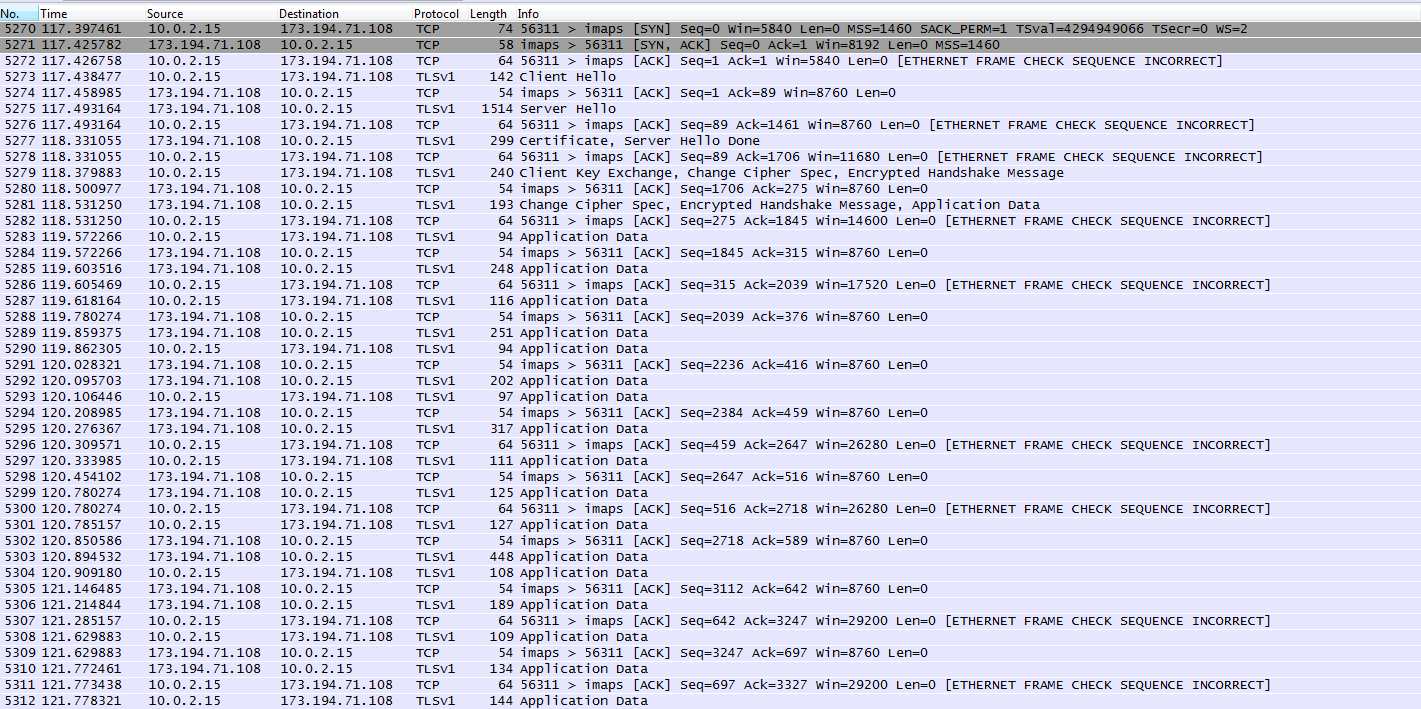
\includegraphics{ws1}
\end{center}
\end{figure}

\begin{figure}[h!]
\begin{center}
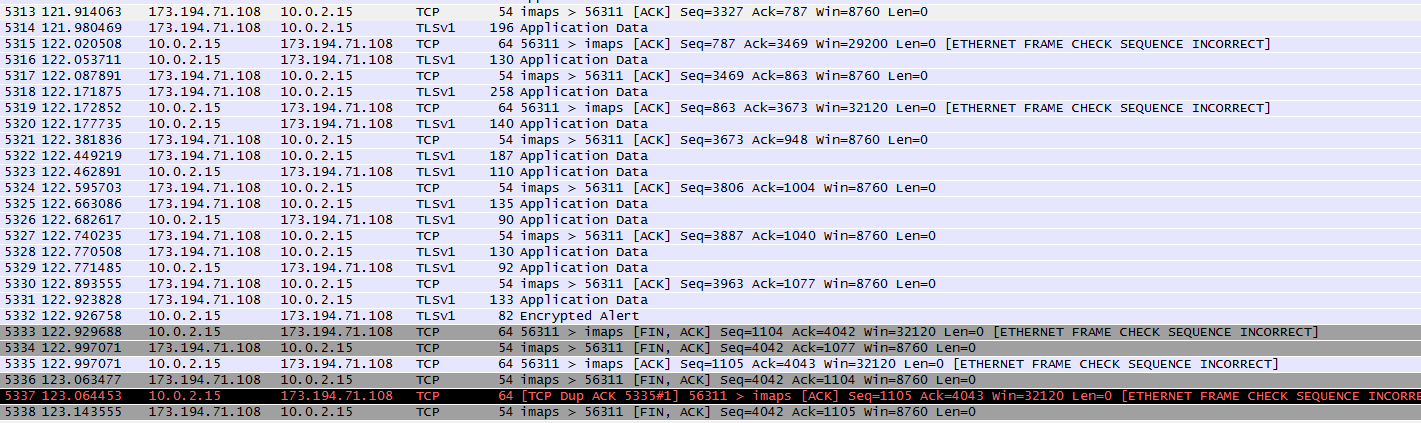
\includegraphics{ws2}
\end{center}
\end{figure}

See table \ref{tab:summaryrecmes} at page \pageref{tab:summaryrecmes}.
\begin{table}
\begin{tabular}{ll} \hline
Packets & 69 \\
Time between first and last package & 5.746 seconds \\
Average packets per second & 12.008 \\
Average packet size & 131 000 bytes \\
Bytes & 9039 \\
Average bytes per second & 1573.069 \\
Average Mbit per second & 0.013 \\ \hline
\end{tabular}
\caption{Summary of the event of receiving a message} \label{tab:summaryrecmes}
\end{table}

The following Wireshark screenshot only includes the TLS packets sent to and from our application.

\begin{figure}[h!]
\begin{center}
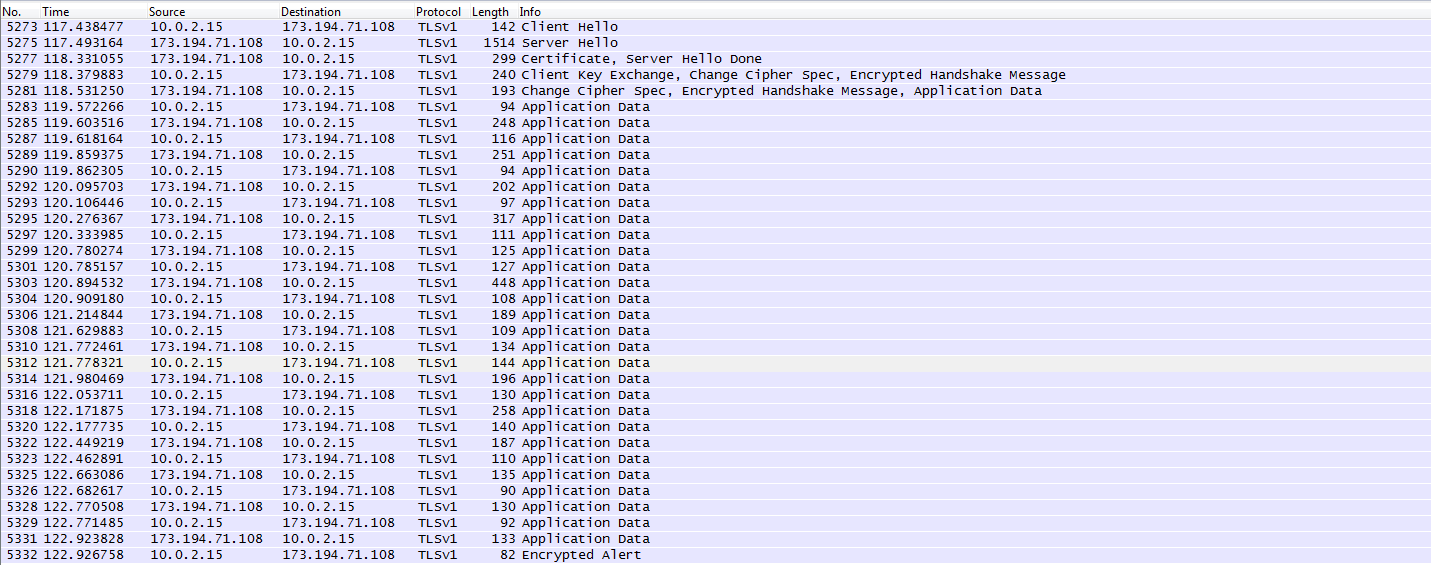
\includegraphics{ws3}
\end{center}
\end{figure}

After investigating the Wireshark capture we could see that receiving a message acts according to the TLS protocol with one exception. The handshake between the client and the server is performed according to the rules of the protocol, except the \textbf{Finished}  message is never sent from either part, instead there appears to be an \textbf{Encrypted Alert}. This does not seem to be a problem as the application ends the IMAP connection shortly after and thus closing the connection. The encrypted alert could be a normal “close notify” message.
\newline
\newline
When considering the amount of data sent and the time it takes to send it, we can see that the data exchanged between the client and server is 8992 Bytes and that it takes 5.384 seconds to finish the session. This is not bad considering that the information was transferred over GSM bandwidth. The actual message itself was 990 bytes but the application data sent from the server was 2953 bytes. This increased the data transferred by 66.47\% During the receiving of this message there were only one duplicate packet.

\subsection{Sending a message}

The following two screenshots from Wireshark contains all the traffic going to and from our application when sending a single message from our application.

\begin{figure}[h!]
\begin{center}
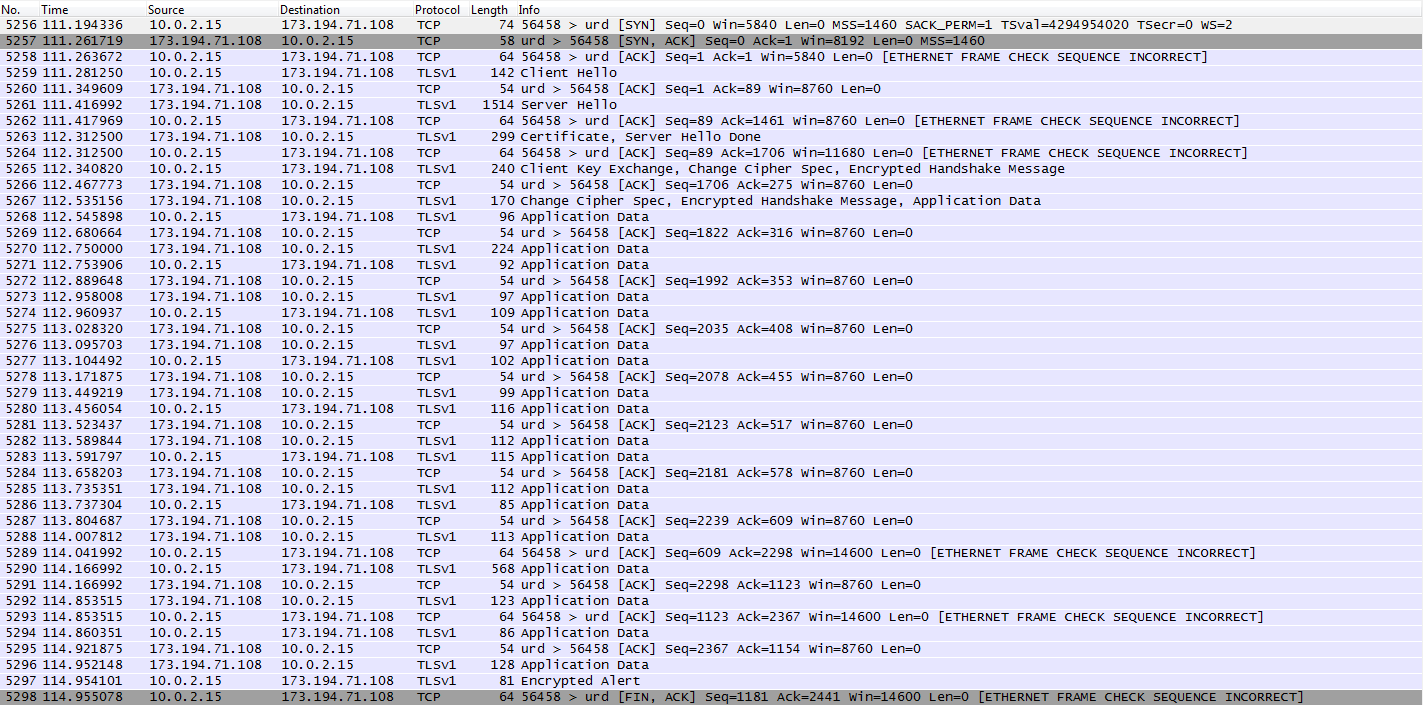
\includegraphics{ws4}
\end{center}
\end{figure}

See table \ref{tab:summarysenmes} at page \pageref{tab:summarysenmes}.
\begin{table}
\begin{tabular}{ll} \hline
Packets & 648 \\
Time between first and last package & 4.056 seconds \\
Average packets per second & 11.835 \\
Average packet size & 131 667 bytes \\
Bytes & 6320 \\
Average bytes per second & 1558.314 \\
Average Mbit per second & 0.012 \\ \hline
\end{tabular}
\caption{Summary of the event of sending a message} \label{tab:summarysenmes}
\end{table}

The following Wireshark screenshot only includes the TLS packets sent to and from our application.

\begin{figure}[h!]
\begin{center}
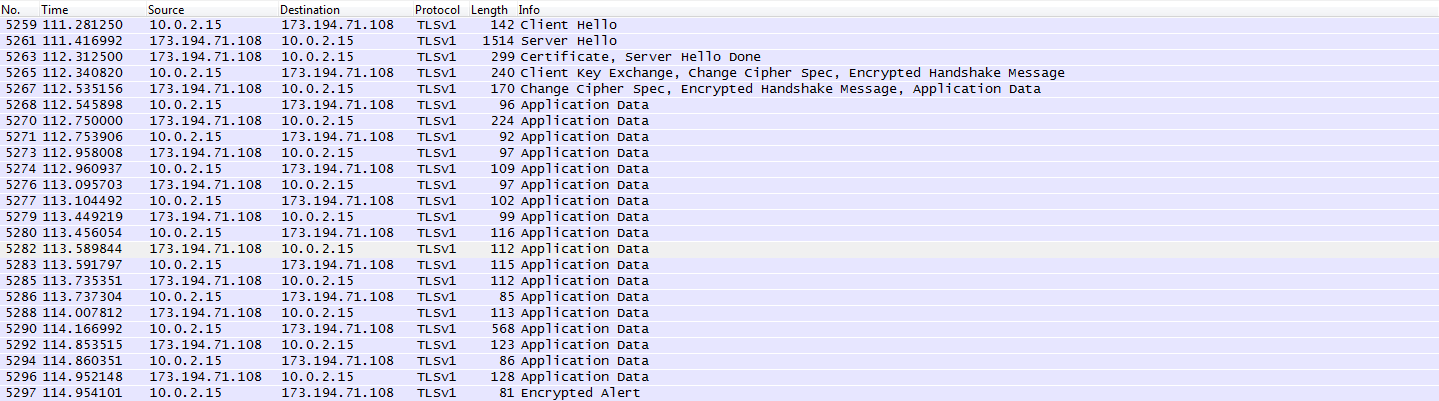
\includegraphics{ws5}
\end{center}
\end{figure}

When sending a message from the application it acts in a similar manner to the receiving part. It follows the TLS protocol with the same \textbf{Encrypted Alert} message at the end instead of the server and client \textbf{Finished} message. 
\newline
\newline
Sending a single message takes 4.056 seconds and transfers 6320 bytes between the server and client. This is not bad for a GSM connection. The message sent from the client to the server had a size of 3150 bytes. The data sent from the client to the server was 1348 bytes.
This is an increase of data by 42.7%. During this transmission there was only one duplicate packet sent from the client to the server.
